\documentclass[twocolumn]{aastex63}


\usepackage{graphicx}	% Including figure files


\let\tablenum=\undef % This fixes an incompatibility between aastex and siunitx
\usepackage{siunitx}
\sisetup{
  % explicit""+" is useful for velocities
  retain-explicit-plus = true,
  % prefer 10^6 over 1 x 10^6
  retain-unity-mantissa = false,
  % Use x +/- e instead of x(e)  
  separate-uncertainty = true,
  % Make sure to pick up bold font when used in section heading for instance
  detect-weight = true,
}

\newcommand{\vdag}{(v)^\dagger}
\newcommand\aastex{AAS\TeX}
\newcommand\latex{La\TeX}

\newcommand{\eduardo}[1]{{\color{teal}E: #1}}
\newcommand{\jorge}[1]{{\color{magenta}J: #1}}
\newcommand{\cesar}[1]{{\color{red}C: #1}}
\newcommand{\Karla}[1]{{\color{violet}K: #1}}
%% Reintroduced the \received and \accepted commands from AASTeX v5.2
\received{XXX}
\revised{YYY}
\accepted{ZZZ}
%% Command to document which AAS Journal the manuscript was submitted to.
%% Adds "Submitted to " the argument.
\submitjournal{ApJ}
\shortauthors{M\'endez-Delgado et al.}

\graphicspath{{./}{figures/}}
%% This is the end of the preamble.  Indicate the beginning of the
%% manuscript itself with \begin{document}.


\begin{document}

\title{Photoionized Herbig-Haro objects in the Orion Nebula through deep high-spectral resolution spectroscopy II: HH~204}


\shorttitle{HH~204 in the Orion Nebula}



\correspondingauthor{Jos\'e E. M\'endez-Delgado}
\email{jemd@iac.es}

\author[0000-0002-6972-6411]{J. E. M\'endez-Delgado}
\affiliation{Instituto de Astrof\'isica de Canarias (IAC), E-38205 La Laguna, Spain}
\affiliation{Departamento de Astrof\'isica, Universidad de La Laguna, E-38206 La Laguna, Spain}


\author[0000-0002-5247-5943]{C. Esteban}
\affiliation{Instituto de Astrof\'isica de Canarias (IAC), E-38205 La Laguna, Spain}
\affiliation{Departamento de Astrof\'isica, Universidad de La Laguna, E-38206 La Laguna, Spain}


\author[0000-0002-6138-1869]{J. Garc\'ia-Rojas}
\affiliation{Instituto de Astrof\'isica de Canarias (IAC), E-38205 La Laguna, Spain}
\affiliation{Departamento de Astrof\'isica, Universidad de La Laguna, E-38206 La Laguna, Spain}


\author[0000-0001-6208-9109]{W. J. Henney}
\affiliation{Instituto de Radioastronom\'ia y Astrof\'isica, Universidad Nacional Aut\'onoma de M\'exico, Apartado Postal 3-72, 58090 Morelia, Michoac\'an, Mexico}

\author[0000-0003-3776-6977]{A. Mesa-Delgado}
\affiliation{Calle Camino Real 64, Icod el Alto, Los Realejos, 38414, Tenerife, Spain}

\author[0000-0002-2644-3518]{K. Z. Arellano-C\'ordova}
\affiliation{The University of Texas at Austin, 2515 Speedway Boulevard Stop C1400, Austin, TX 78712, USA}


\received{XXX}
\revised{YYY}
\accepted{ZZZ}

%\nocollaboration{1}



%\collaboration{1}{(LaTeX collaboration)}

%\nocollaboration{2}

%% Note that the \and command from previous versions of AASTeX is now
%% depreciated in this version as it is no longer necessary. AASTeX 
%% automatically takes care of all commas and "and"s between authors names.

%% AASTeX 6.3 has the new \collaboration and \nocollaboration commands to
%% provide the collaboration status of a group of authors. These commands 
%% can be used either before or after the list of corresponding authors. The
%% argument for \collaboration is the collaboration identifier. Authors are
%% encouraged to surround collaboration identifiers with ()s. The 
%% \nocollaboration command takes no argument and exists to indicate that
%% the nearby authors are not part of surrounding collaborations.

%% Mark off the abstract in the ``abstract'' environment. 
\begin{abstract}

Contribuciones de Will para el artículo

\end{abstract}

%% Keywords should appear after the \end{abstract} command. 
%% See the online documentation for the full list of available subject
%% keywords and the rules for their use.
\keywords{ISM:Abundances – ISM: Herbig–Haro objects – ISM: individual:
Orion Nebula – ISM: individual: HH 204}

\section{Material de Will}
\label{sec:will}

\newcommand\chem[1]{\ensuremath{\mathrm{#1}}}
\newcommand\ha{\ensuremath{\mathrm{H\alpha}}}
\newcommand\hb{\ensuremath{\mathrm{H\beta}}}
% aastex \ion command is useless - must replace it
\newcounter{ionstage}
\renewcommand{\ion}[2]{\setcounter{ionstage}{#2}% 
  \ensuremath{\mathrm{#1\,\scriptstyle\Roman{ionstage}}}}
\newcommand\oiii{[\ion{O}{3}]}
\newcommand\siii{[\ion{S}{3}]}
\newcommand\nii{[\ion{N}{2}]}
\newcommand\wav[1]{\ensuremath{\lambda #1}}
\newcommand\Te{\ensuremath{T_{\mathrm{e}}}}
\newcommand\BG{\ensuremath{_{\mathrm{BG}}}}
% Stars in Orion, e.g., \th1C, \th2A
\def\th#1#2{\ensuremath{\theta^{#1}\,\text{Ori~#2}}}


 
\begin{figure}
  \centering
  \includegraphics[width=\linewidth]{hh204-finding-chart-simple}
  \caption{
    Location of the UVES spectrograph slit at the head of the HH~204 bow shock.
    The background RGB images shows the immediate environs of HH~203 and 204,
    derived from \textit{HST} WFPC2 observations \citep{ODell:1996a} in filters of
    \oiii{} (red), \nii{} (green), and \ha{} (blue).
    }
  \label{fig:hh204-finding-chart-simple}
\end{figure}


\begin{figure*}
  \centering
  \includegraphics[width=\textwidth]{hh204-ratio-oiii-ha-annotated}
  \caption{
    (a) Map of the line ratio \(\oiii{}\ \wav{5007} / \ha\ \wav{6563}\),
    calculated from \textit{HST} images with the PC chip of the WFPC2 camera.
    The position of the UVES spectrograph slit is outlined by a dashed box,
    while a further region of interest in the N wing of the bow shock
    is indicated by a dotted box.
    The vertically oriented ``scar'' at upper left is an artifact
    due to the bright star \th2A, located just north of the field of view.
    (b)~Average cut profiles of the \textit{HST} images for the box in the N wing
    that is outlined in panel~a.
    Upper graph shows surface brightness profiles in the two emission lines,
    normalized to the mean nebular background value outside of the shock.
    Lower graph shows the line ratio,
    with the raw ratio indicated by the black solid line
    and the background-subtracted ratio indicated by the gray histogram.
    The zero point of the displacement axis is taken to be the location
    of the maximum gradient in the \ha{} surface brightness.
    (c)~Same as panel~b, but showing average profiles of the \textit{HST} images
    along the UVES slit.
    The region of the slit that
    shows \(\Te(\oiii) > \SI{12000}{K}\) in the blueshifted component
    is indicated by the red arrow.
  }
  \label{fig:ratio-hst-oiii-ha}
\end{figure*}

\textbf{Pongo primero lo de \textit{HST} porque es más completo.}

\subsection{Sub-arcsecond imaging of HH 204}
\label{sec:high-resol-imag}

Figure~\ref{fig:ratio-hst-oiii-ha}a shows the ratio of surface brightnesses,
\(R(\oiii) = S(\oiii\ \wav{5007}) / S(\ha\ \wav{6563})\),
calculated from \textit{HST} WFPC2
observations in the F502N, F547M, F656N, and F658N filters
from program GO5469 \citep{ODell:1996a}.
Flux calibration and correction for contamination by continuum and non-target lines
was performed using the coefficients given in \citet{ODell:2009b}.
It can be seen that the line ratio in the background nebula shows a pronounced gradient
from \(R(\oiii) \approx 0.3\) in the north-east
to \(R(\oiii) \approx 0.5\) in the south-west.%
\footnote{
  For comparison with results from our UVES spectra,
  and using the average reddening for the HH~204 region \citep{Weilbacher:2015a},
  the conversion is \(\wav{4959} / \hb \approx 1.1 R(\oiii)\).
}
Inside the bow shock, the ratio is significantly smaller,
for instance falling from \(\simeq 0.4\) to \(\simeq 0.2\) along the length of the UVES slit.

However, the most interesting feature of the \(R(\oiii)\) image is the slight
\emph{increase} in the ratio that is seen
in a thin layer along the leading edge of the bow shock.
This is most clearly visible in the northern wing of HH~204,
such as the area highlighted by a dotted outline box in the figure.
Average profiles across the shock for this region
are shown in Figure~\ref{fig:ratio-hst-oiii-ha}b.
The lower panel shows that the raw ratio (solid black line) increases only slightly
above its value in the background nebula,
which is because the brightness increase across the bow shock is
only a small fraction of the background brightness, as can be appreciated in the upper panel.
In order to isolate the emission of the shocked gas from that of the nebula,
we calculate the background-subtracted line ratio:
\begin{equation}
  \label{eq:ratio-bg-sub}
  R'(\oiii) = \frac{S(\oiii) - S\BG(\oiii)}{S(\ha) - S\BG(\ha)}
\end{equation}
under the assumption that \(S\BG\) for each line is constant along the profile.
The result is shown as a gray histogram in the lower panel of the figure,
which reveals a sharp peak of width \(\approx \SI{0.3}{mpc}\)
that reaches a maximum value \(R'(\oiii) \approx 2 R\BG(\oiii)\)
and is centered on a displacement of \(\approx \SI{-0.1}{mpc}\).
The origin of the displacement axis is set to the peak
in the spatial gradient of the \ha{} surface brightness,
corresponding to the outer edge of the dense shocked shell.
The negative displacement of the \(R'(\oiii)\) peak means that this occurs
\emph{outside} the dense shell, closer to the shock front itself. 

Figure~\ref{fig:ratio-hst-oiii-ha}c shows the same quantities
calculated along a cut that coincides with our UVES slit at the head of HH~204.
In this case, \(R'(\oiii)\) is always significantly less than \(R\BG(\oiii)\),
but it does still show a small local peak with a position and width
that is similar to the more impressive one in the northern wing.
These peaks in \(R'(\oiii)\) occur over a much smaller scale than
any of spatial gradients that we find in our UVES slit spectra
and are only detectable because of the high spatial resolution of the \textit{HST}.%
\footnote{
  Pixel size of \SI{0.045}{arcsec},
  which well samples the PSF width at \ha{} of \SI{0.083}{arcsec}.
}
For example, the increase in \(\Te(\oiii)\)
that we detect in the blue-shifted emission near the shock front
(Figure~6)
occurs over a scale of \SI{5}{mpc},
indicated by the red arrow in the figure,
which is more than 10 times larger than the width of the \(R'(\oiii)\) peak.

\textbf{Lo que sigue es más bien discusión}

What is the origin of the narrow peak in the \(\oiii/\ha\) ratio
that is seen just outside the shocked shell?
When a shock propagates into low-ionization gas (predominantly \chem{O^+}),
there are three zones where enhanced \oiii{} emission might be expected
\citep{Cox:1985a, Sutherland:2017a}:
first, the radiative precursor in the pre-shock gas;
second, the non-equilibrium collisional ionization zone immediately after the shock;
third, the radiative relaxation zone where the post-shock gas cools back down
to the photoionization equilibrium temperature of \(\sim \SI{e4}{K}\).
The first of these can be ruled out in the case of HH~204
because the pre-shock photoionization of \chem{O^+} would require shock velocities
greater than \SI{150}{km.s^{-1}},
observed proper motion and radial velocities imply a shock velocity less than \SI{100}{km.s^{-1}}.
% (\textit{Check the exact number.  All the shock papers only give the velocity to pre-ionize hydrogen.})
The second zone has a high temperature
(\( > \SI{50 000}{K}\) for shock velocities \(> \SI{55}{km.s^{-1}}\))
but is severely under-ionized, resulting in line emissivities
that are far in excess of the equilibrium values in a very thin layer.
% However, the region that can emit \oiii{} lines
% is likely to be extremely thin due to the high collisional ionization rate
% (\textit{make an estimate of the thickness}).
The third zone, in which oxygen is recombining through the \chem{O^{++}} stage
while cooling through the range \SI{30000}{K} to \SI{10000}{K}
is predicted to be somewhat thicker and with a higher electron density,
yielding a greater contribution to the total \oiii{} emission.
Given the electron density that we derive of \SI{13500}{cm^{-3}} (Table~3),
and assuming a shock velocity \(< \SI{70}{km.s^{-1}}\),
the cooling length should be approximately \SI{0.05}{mpc},
or \SI{0.025}{arcsec}, which is a few times smaller than the \textit{HST} resolution.
However, this analysis applies only to the head of the bow shock.
In the wings, the shock is not perpendicular to the upstream gas velocity,
but is oblique at an angle \(\alpha\).
This yields a post-shock equilibrium density that is smaller by a factor of \(\cos^2\alpha\),
and a cooling length that is larger by the same factor.
Hence, the cooling length is expected to be resolved for \(\alpha\) smaller than about \ang{45},
which is consistent with our observations of the narrow peak in
the \(\oiii/\ha\) ratio in the north wing.
The reason that the same behaviour is not seen in the opposite wing is probably
that the ambient nebular emission is much more highly ionized there,
which masks the effect.


% \textit{Calculate the cooling length and show that in the wings,
%   where the post-shock density is less than \SI{e4}{cm^{-3}}, we should
%   resolve the cooling zone, whereas at the bow shock head
%   where the density is greater than \SI{2e4}{cm^{-3}}, it will be unresolved.
%   This may explain why we only clearly see the peak in \(R'(\oiii)\) in the wing.
%   (But this may also be due to dilution by the Mach disk, see below).
% }

\newcommand\Mach{\ensuremath{\mathcal{M}}}
Note that the length scales over which we see changes in \(T(\oiii)\) from the UVES data
are much larger than this (\(\approx \SI{5}{mpc}\), see Figure~7),
and so cannot be ascribed to the cooling zone behavior described above.
Instead, we suggest that we are seeing the superposition of two different emission
components: one from the bow shock and one from the Mach disk (the shock internal to the jet).
The jet shock will have a lower Mach number, \(\Mach\), than the bow shock
so long as the unshocked jet is denser than the ambient medium,
as appears to be the case in HH~204.
The thickness of the equilibrium (cooled) shocked shell is proportional to \(\Mach^{-1}\)
and so should be larger for the shell behind the Mach disk, which thus dominates the
emission in much of the slit (displacements \num{5} to \SI{12}{mpc} in Figure~7).
At smaller displacements, the contribution of the bow shock gets progressively larger,
thus explaining the increase in \(T(\oiii)\).
The expected length scale for this variation is roughly the radius of curvature of the bow shock,
which agrees with the observed \SI{5}{mpc}.
The only reason that this effect is visible at all is that \oiii{} emission from the
equilibrium shell is so weak.
For lower ionization lines, the contribution of the bow shock to the total brightness
is always negligible, even for positions close to the shock.

% \textit{Then, how to explain the behavior of \(\Te(\oiii)\),
%   which varies on much larger scales than the cooling length.
%   Possibly related to the radius of curvature of the shock.
%   Alternatively, could be that we are seeing a mixture
%   of the two shocked shells:
%   the one from behind the bow shock and the one from behind the Mach disk (jet shock).
%   As we move along the slit away from the shock,
%   the Mach disk shell dominates more and more.
%   If the jet shock is lower velocity than the bow shock,
%   then this might explain the observed gradient in the \oiii{} temperature.
%   This is also consistent with the appearance of the object:
%   there is a big clump of emission that disappears once you move away from the axis into the wings,
%   while the bow shock part remains.
% }


\begin{figure*}
  \centering
  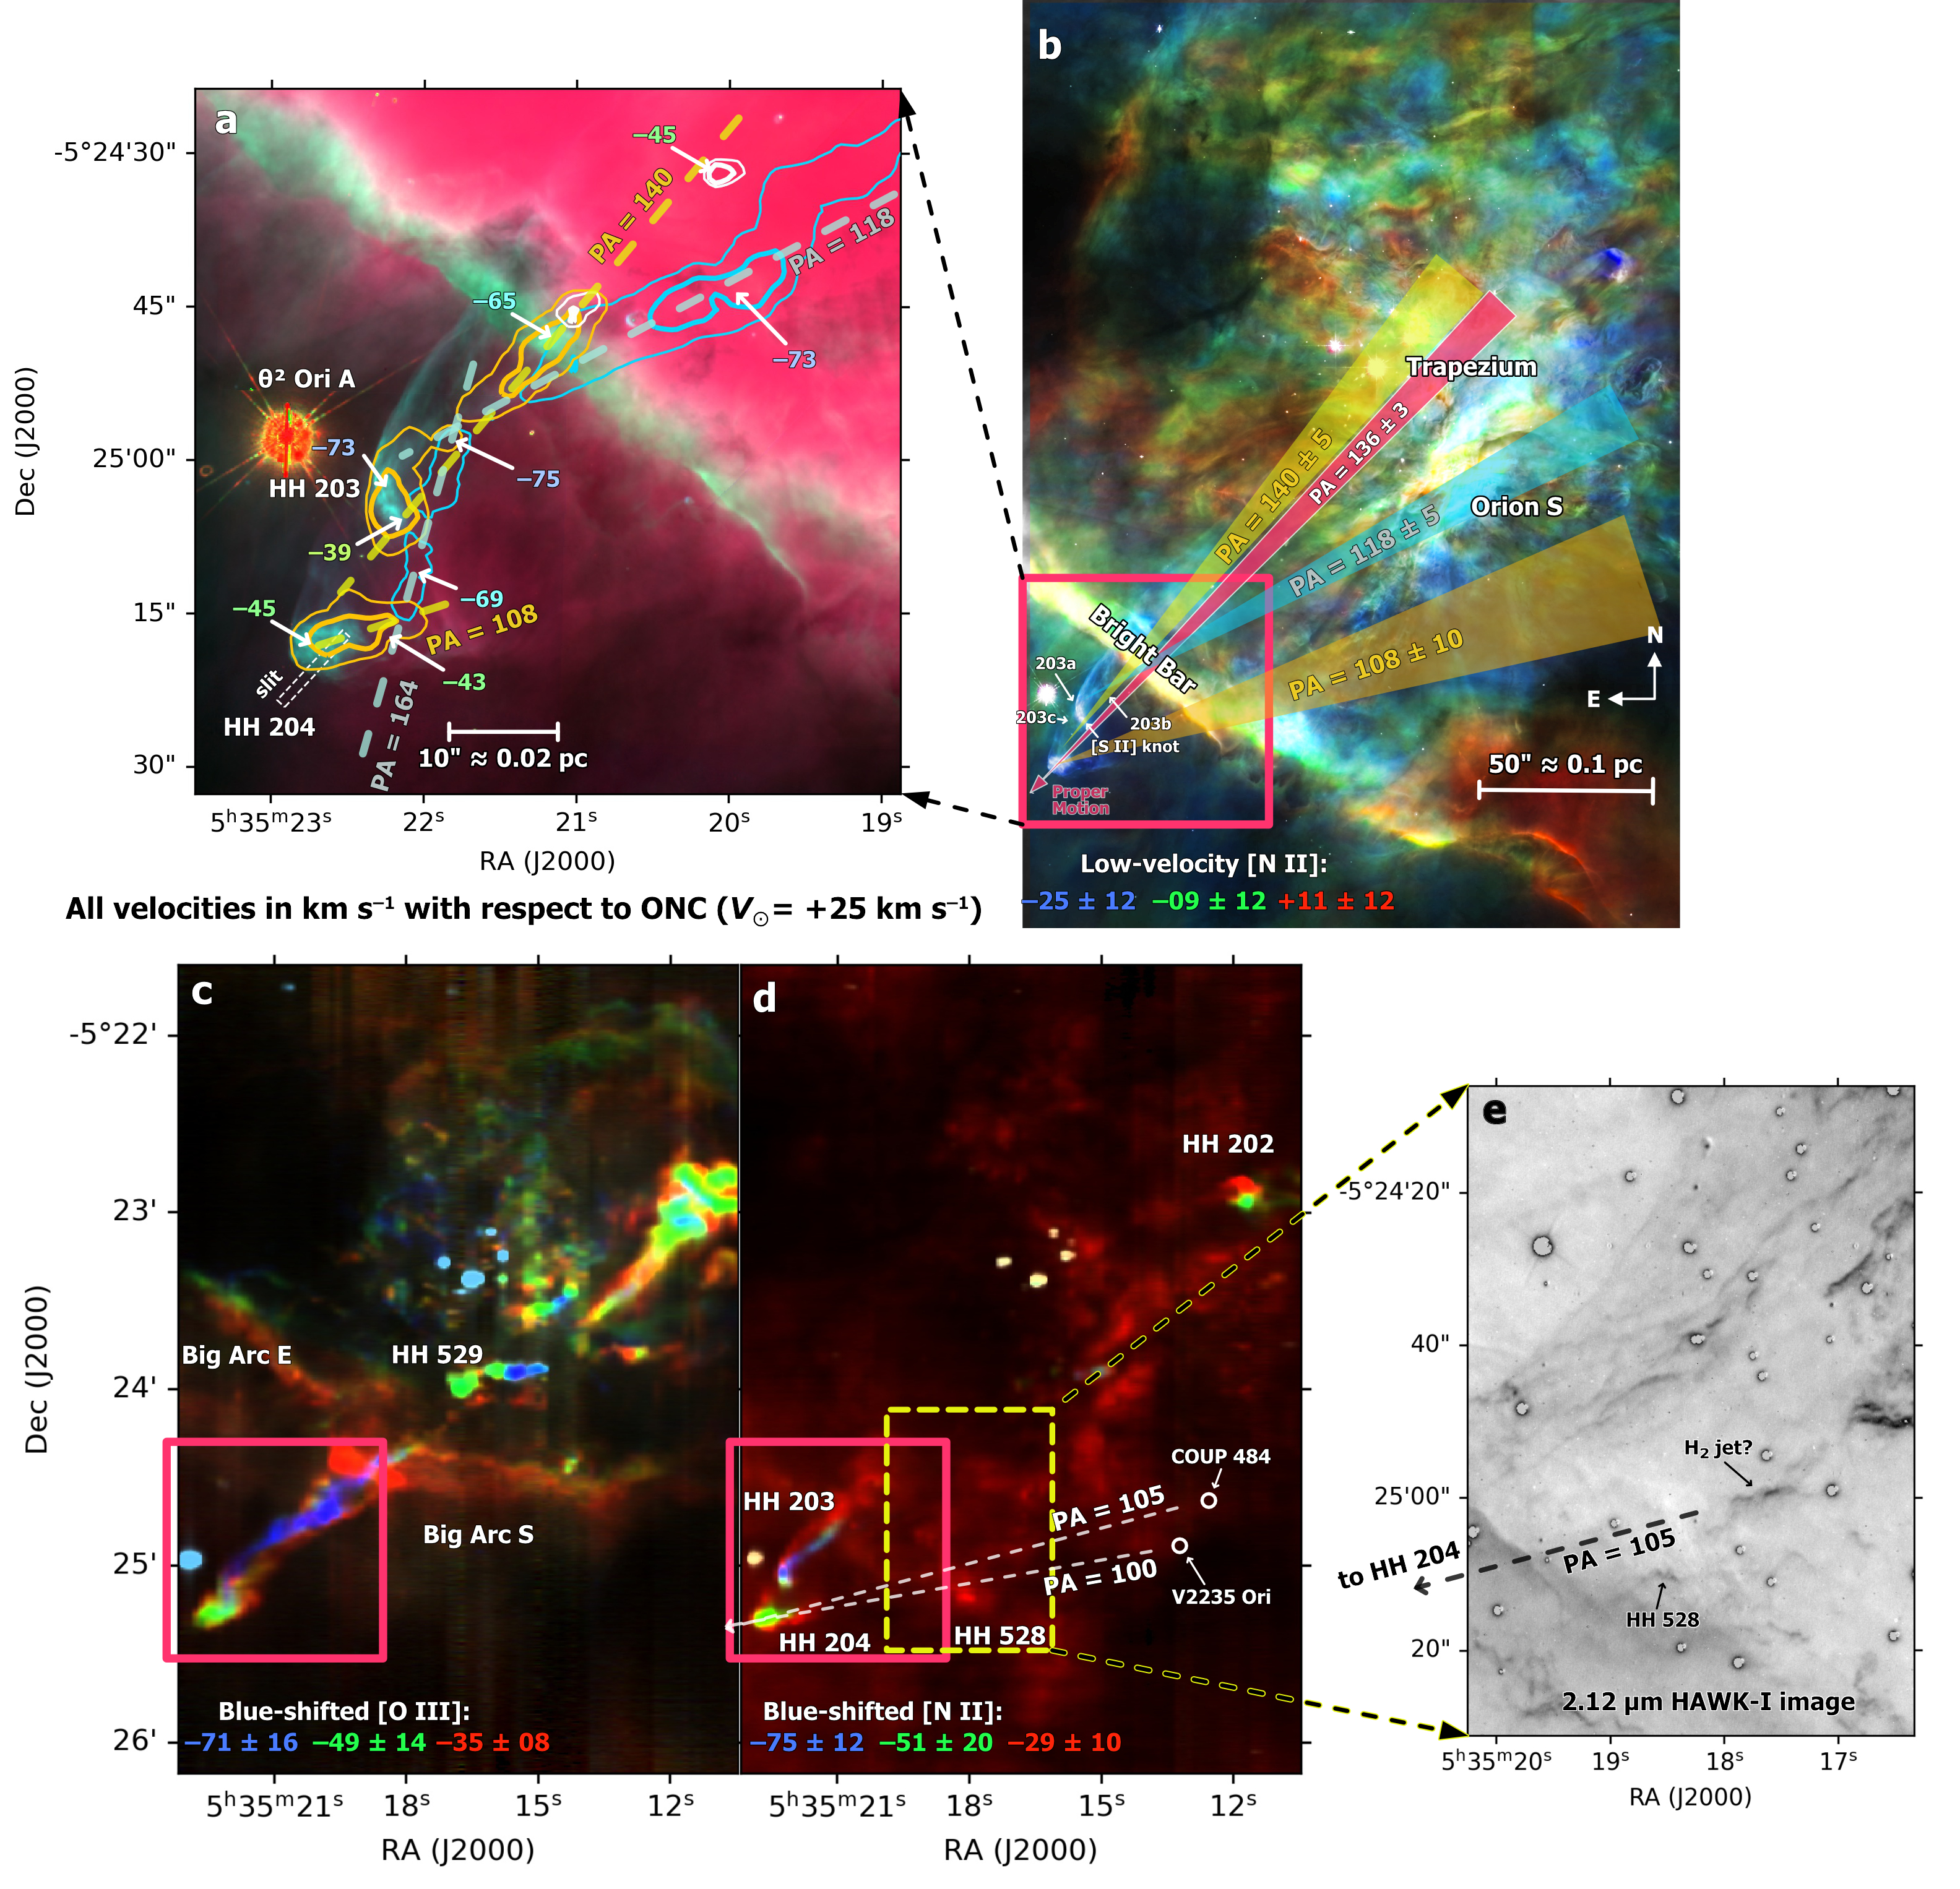
\includegraphics[width=\textwidth]{hh204-finding-chart}
  \caption{Location of HH~204 within the Orion Nebula.
    (a)~Same as Figure~\ref{fig:hh204-finding-chart-simple}
    but showing an expanded view of the bow shocks and possible driving jets.
    Contours show highly blue-shifted emission of \oiii{}
    (cyan, centered on \SI{-70}{km.s^{-1}})
    and \nii{}
    (yellow, centered on \SI{-50}{km.s^{-1}}, and white, centered on \SI{-35}{km.s^{-1}}),
    derived from multiple longslit spectra
    \citetext{\citealp{Doi:2004a}
      as recalibrated in spectral atlas of \citealp{Garcia-Diaz:2008a}}.
    Mean velocities with respect to the Orion Nebular Cluster
    of particular features related to the HH objects are indicate by arrows.
    (b)~Location of HH~204 with respect to the inner Orion Nebula.
    The intensity of the image comes from the \nii{} \textit{HST} WFPC2 observations,
    but colorized according to the velocity of the slow-moving nebular gas
    (within about \SI{30}{km.s^{-1}} of the systemic velocity) as derived from the
    longslit spectra, see color key on figure.
    (c)~Highly blue-shifted \oiii{} emission for a field of view similar to that of panel~b.
    (d)~As panel~c but for highly blue-shifted \nii{} emission.
    Two candidate stellar sources along the back-projection of the PA108 flow
    are indicated by white circles (see discussion in text).
    (e)~Near-infrared HAWK-I imaging
    of the region outlined by a yellow dashed box in panel~d
    in the \SI{2.12}{\micro m} \chem{H_2} line \citep{Kissler-Patig:2008a},
    showing an emission filament that may be associated with HH~204.
    }
  \label{fig:hh204-finding-chart}
\end{figure*}

\subsection{Origin of the jet that drives HH 204}
\label{sec:origin-jet-that}

At least two different high-velocity flows
converge on the general HH~203/204 region
from the direction of the inner Orion Nebula (see Figure~\ref{fig:hh204-finding-chart}),
but it is not clear if either of them are directly responsible for driving the
HH~204 bow shock.
One flow is at a position angle (PA) of \(\approx \ang{118}\) and transitions 
from a high ionization state north-west of the Bright Bar
(cyan contours in Fig.~\ref{fig:hh204-finding-chart}a),
to a lower ionization state (yellow contours) to the south-east of the Bright Bar.
The other is at \(\mathrm{PA} \approx \ang{140}\)
and is of low ionization for its entire detected length. 
Both these flows give the appearance of driving HH~203,
which implies that HH~203 may be a superposition of two unrelated bow shocks.
Such a superposition is consistent with the detection of two
different velocity components (\num{-73} and \SI{-39}{km.s^{-1}})
at the head of the bow shock, and also with the complex structure
apparent in high-resolution \textit{HST} images (see Fig.~\ref{fig:hh204-finding-chart}b).
\citet{ODell:2015a} noted that in addition to the main bow shock (HH~203a),
there appears to be a second faint bow shock (HH~203b), associated with
the PA118 flow.
We also detect a third faint bow shock, which we denote HH~203c,
situated in front (SW) of HH~204a.
Note that \citet{ODell:2015a} give position angles of \ang{124} and \ang{127},
respectively, for HH~203 and HH~204, which probably represent an average of the 
PA118 and PA140 flows. 

The southern portion of HH~203a,
which we label as ``[\ion{S}{2}] knot'' in the figure,
is particularly strong in the [\ion{S}{2}] and [\ion{O}{1}] filters
and coincides with the peak of the \SI{-39}{km.s^{-1}} feature.
The spatial alignment and the similarity in velocity and ionization makes it likely that this
knot is part of the PA140 flow.
It is conceivable that this flow may extend farther to the SW and
be driving the HH~204 bow shock,
although there is no direct evidence for this.
On the other hand, a third flow at \(\mathrm{PA} \approx \ang{108}\) is seen to feed into HH~204
from the west.
This jet, first noted by \cite{Doi:2004a}, is very short and stubby,
and can be traced back only \SI{10}{arcsec} (\SI{20}{mpc}) from the bow shock.
There is another faint filament of high-velocity \oiii{} emission that extends between the
HH~203 and HH~204 regions at \(\mathrm{PA} \approx \ang{108}\)
(see Fig.~\ref{fig:hh204-finding-chart}a).
This appears to provide a connecting bridge
between the PA140 and PA108 flows, although the difference
in velocity and ionization with respect to the PA108 flow argues against
a physical association with HH~204. 

We have searched archival observations in other wavebands
for any evidence of jets along the back projection of the PA108 axis.
The most convincing association is with a molecular hydrogen filament
seen in the \SI{2.12}{\micro m} line (see Figure~\ref{fig:hh204-finding-chart}e).
At the position of this filament, HH~204 is at \(\mathrm{PA} = \ang{105}\),
which is well within the uncertainties,
and the orientation of the filament is consistent with the same PA.\@
Unfortunately, no kinematic observations are currently available for this filament,
so its association with HH~204 can only be tentative.
The stellar source that best aligns with the \chem{H_2} filament
is COUP~484, see Figure~\ref{fig:hh204-finding-chart}e.
However, this is a rather low luminosity star and therefore seems
an unlikely candidate for driving such an impressive large-scale outflow.
The star V2235~Ori is also marginally consistent within the uncertainty
with the PA108 axis and is roughly 100 times brighter than COUP~484
in the K and L infrared bands \citep{Muench:2002a},
but its position is completely inconsistent with being the source of the \chem{H_2} filament.
There is also marginal evidence from MUSE observations \citep{Weilbacher:2015a}
for a blue-shifted [\ion{Fe}{3}] filament that extends
from the position of the \chem{H_2} filament towards HH~204, but the data are noisy. 

A further important line of evidence for the flow direction is provided
by proper motion measurements.
We have re-measured the proper motions using \emph{HST} images over an interval of 19 years (1996 to 2015) using the methodology described in section~10 of Paper~I.
For the ``nose'' of the HH~204 bow shock, we find a plane-of-sky velocity of \SI{71 \pm 9}{km.s^{-1}}
at \(\mathrm{PA} = \ang{136 \pm 3}\).
After correcting to a common distance of \SI{417}{pc}
the previous measurements of \citet{Doi:2002v} are \SI{83 \pm 10}{km.s^{-1}}
at \(\mathrm{PA} = \ang{137 \pm 7}\),
which are consistent with our measurements within the uncertainties.
The proper motion axis is shown by a large red arrow in Figure~\ref{fig:hh204-finding-chart}b
for comparison with the candidate axes from the high radial velocity jets.
It is marginally consistent with the PA140 axis, but not all with the
PA108, PA118, or PA164 axes. 

In summary, convincing evidence for which large scale flow might be driving the
HH~204 bow shock is frustratingly absent.
Although the PA108 flow is clearly associated with HH~204, its short length means
that the exact orientation is very uncertain.
The PA140 flow has a much better defined direction,
but its extension beyond the position of the [\ion{S}{2}] knot
in order to feed into the HH~204 bow shock is purely speculative.
However, the close agreement between this flow direction
and the proper motion axis is an additional argument in its favor.
The only thing that can be said with any degree of certainty is that the
high-ionization PA118 flow is \emph{not} driving HH~204, but only HH~203.

In Figure.~\ref{fig:hh204-finding-chart}b we show the back projection of
all three of these flows into the core of the nebula,
assuming an uncertainty of \ang{\pm 10} for the PA108 flow
and \ang{\pm 5} for the other two.
The PA118 flow is consistent with an origin in the Orion~S
star forming region,
as has been remarked many times previously
\citep{ODell:1997a, Rosado:2002e, ODell:2003n}.
However, neither of the other flows are consistent with an origin in that region,
unless the flow has suffered a relatively large-angle deviation.
The back-projection of the PA108 flow falls significantly to the south
of the main Orion~S region
in an area with no convincing candidates for the driving source
(see above discussion of the possible \chem{H_2} jet).
The back-projection of the PA140 flow intersects the Trapezium stars
in the very center of the nebula, which raises the possibility that the source
may be a proplyd, which are highly concentrated in that region.

% 5:35:14.2753 -5:24:24.958 => 143-425 V1328 Ori

\clearpage

\section{Two-zone model for observed temperature structure}

\newcommand\zA{\ensuremath{_\mathrm{A}}}
\newcommand\zB{\ensuremath{_\mathrm{B}}}

At each position along the spectrograph slit, the line of sight will cross several zones
with different physical conditions.  These may include:
\begin{description}
\item[A1] The compressed shell behind the bow-shock,
  which is in photoionization equilibrium;
\item[A2] The main body of the jet bullet, also in photoionization equilibrium;
\item[B1] The immediate post-shock cooling zone of the bow shock;
\item[B2] The post-shock cooling zone of the jet shock.
\end{description}
In HH~204, the relative velocity between the unshocked jet and the working surface
is very low (\(\approx \SI{15}{km.s^{-1}}\)), so the jet shock is much weaker than the bow shock,
implying that the emission from zone B2 can be neglected compared with B1.
Zones A1 and A2 should have similar conditions, and so can be merged into a single zone with density \(n\zA\) and temperature \(T\zA\).
Although the zone B1 should have a range of temperatures,
for simplicity we assume a single characteristic temperature \(T\zB\).
The density of zone B is found by assuming pressure equilibrium with zone A:
\(n\zB = n\zA T\zA / T\zB\).
We define \(f\zB\) for a given ion as the fraction of the total ionic emission measure,
\(\int n_{\mathrm{e}}\, n_{\mathrm{ion}}\,dz\),
that comes from zone~B,
with the remainder, \(f\zA = 1 - f\zB\), coming from zone~A.

The appropriate value of \(T\zB\) is rather uncertain,
since it depends on the non-equilibrium evolution of ionization and temperature
in the post-shock radiative relaxation layer.
Most published shock models \citep{Cox:1985a, Sutherland:2017a}
are calculated on the assumption that the
far upstream and downstream ionization states are determined by the radiation from the shock itself.
Care must therefore be exercised when translating their results to cases such as HH~204,
where external irradiation from O~stars is a dominant factor.
The curved bow shock in HH~204 should give a range of shock velocities,
up to a maximum of \(V \approx \SI{84}{km.s^{-1}}\) (assuming the pre-shock medium is stationary).
In principle, this corresponds to post-shock temperatures as high as \SI{2e5}{K},
but the gas at such temperatures will be too highly ionized to significantly emit optical lines.
The cooling timescale is generally shorter than the recombination timescale,
so the gas is over-ionized as it cools.
It is only when the temperature falls below about \SI{50000}{K} that the abundance
of \chem{O^{++}} becomes significant \citetext{e.g., Fig.~11 of \citealp{Allen:2008a}},
allowing the emission of the optical [\ion{O}{3}] lines.
A similar situation is seen in middle-aged supernova remnants,
such as the Cygnus Loop \citep{Raymond:2020a}. 

\begin{figure}
  \includegraphics[width=\linewidth]{working-surface-hh204-single}
  \caption{
    A simple model for the principal working surface of the HH~204 jet.
    The shocked gas can be divided conceptually into 4 zones:
    A1, A2, B1, and B2 (see text for details).
  }
  \label{fig:working-surface}
\end{figure}


\begin{figure}
  \textbf{\Large a}\\
  \includegraphics[width=\linewidth]{two-temp-Toiii-Tsiii}\\
  \textbf{\Large b}\\
  \includegraphics[width=\linewidth]{two-temp-TB-30000}
  \caption{
    Simple two-zone model for spatial variations in temperature diagnostics.
    (a)~Correlation between derived \(\Te\) from \oiii{} and \siii{} lines,
    assuming that the fraction \(f\zB\) of ionic emission measure that arises
    in the hot component (with temperature \(T\zB\)) is the same for both ions.
    Values of \(f\zB = 0.01\) (small dots) and \(f\zB = 0.1\) (large dots)
    are indicated on each curve.
    The gray rectangle shows the observed range of values,
    which cannot be explained under this assumption (see text). 
    (b)~Derived \(\Te\) for \oiii{}, \siii{}, and \nii{} lines as a function
    of \(f\zB\), assuming \(T\zB = \SI{30000}{K}\).
    Colored bands show the observed ranges, which imply that \(f\zB(\oiii)\)
    must be larger than for the other ions (see text).
  }
  \label{fig:two-zone}
\end{figure}

We look for solutions where both \(T\zA\) and \(T\zB\) are constant
along the slit,
so that any spatial variation in the temperature diagnostics
is driven primarily by variation in \(f\zB\).
Although the density diagnostics do show a gradient with position,
both \(T(\oiii)\) and \(T(\siii)\) are relatively insensitive to density,
so for simplicity we assume \(n\zA\) is constant.
We use the Python library PyNeb to calculate the per-zone emission coefficients,
\(j(T\zA, n\zA)\) and \(j(T\zB, n\zB)\), for each emission line.
For a given diagnostic line pair, 1 and 2, the ratio is calculated as
\begin{equation}
  \label{eq:2-zone-ratio}
  R_{12} = \frac
  {(1 - f\zB) \, j_1(T\zA, n\zA) + f\zB\, j_1(T\zB, n\zB)}
  {(1 - f\zB) \, j_2(T\zA, n\zA) + f\zB\, j_2(T\zB, n\zB)}.
\end{equation}
This is then fed into PyNeb's \texttt{getTemDen} function
to find the equivalent single-zone temperature that would
give the same ratio (assuming a density of \(n\zA\)).
It is clear from equation~(\ref{eq:2-zone-ratio}) that
for \(f\zB = 0\) one must recover \(\Te = T\zA\) and that
for \(f\zB = 1\) one must recover \(\Te = T\zB\).
But for intermediate values of \(f\zB\),
the derived temperature will differ between ions because
of variations in the temperature sensitivity of the diagnostic ratios.

We first investigate the case of a common \(f\zB\) for all ions,
but we find that this is unable to reproduce the observations.
This is demonstrated in Figure~\ref{fig:two-zone}a,
which shows the relation between \(\Te(\oiii)\) and \(\Te(\siii)\)
for 4 different values of \(T\zB\) between \num{15000} and \SI{50000}{K}.
We set \(T\zA = \SI{9000}{K}\) and \(n\zA = \SI{20000}{cm^{-3}}\) in all cases
and \(f\zB\) increases from left to right along each curve.
The gray rectangle shows the observed range of temperatures
along the spectrograph slit (Figure~6):
\(\Te(\oiii)\) shows a systematic decline from \(\approx \SI{17000}{K}\)
near the bow shock to \(\approx \SI{12000}{K}\) further away,
while \(\Te(\siii)\) is roughly constant at \num{9000} to \SI{10000}{K},
with no apparent correlation with \(\Te(\oiii)\).
The two-zone models with \(T\zB \ge \SI{30000}{K}\)
all show \(\Te(\oiii) > \Te(\siii)\) as \(f\zB\) increases,
but this is insufficient to explain the observations.
For example, in order to achieve \(\Te(\oiii) = \SI{17000}{K}\)
the models predict \(\Te(\siii) > \SI{11000}{K}\),
which is significantly higher than observed.

In Figure~\ref{fig:two-zone}b, we relax the assumption
of a common \(f\zB\) for all ions,
showing separately the predicted values of
\(\Te(\nii)\), \(\Te(\siii)\), and \(\Te(\oiii)\)
as a function of \(f\zB\), assuming \(T\zB = \SI{30000}{K}\).
The ranges of observed values are shown by colored bands,
blue for \oiii{} and orange for \nii{} and \siii{}.
From the figure it is apparent that a decline  
from \(f\zB(\oiii) \approx 0.1\) at \(x = 0\) to
\(f\zB(\oiii) \approx 0.02\) for \(x > \SI{5}{mpc}\)
is required to explain the \(\Te(\oiii)\) profile,
whereas \(f\zB(\siii)) < 0.01\) and \(f\zB(\nii) < 0.01\)
is required at all positions.

It is not surprising that \(f\zB\) should vary between ions
since the photoionization equilibrium ion fraction of \chem{O^{2+}}
from zone~A is much lower than that of \chem{N^{+}} or \chem{S^{2+}}.
Assuming \(f\zB \ll 1\), then the ionic abundances given in
the ``Cut 1, HH 204'' column of Table~4 correspond to zone~A.
These yield \chem{O^{2+} / \chem{O} = 0.005} and
\chem{S^{2+} / \chem{S} = 0.61} if the abundances of unobserved ion stages are negligible.
The lack of [\ion{N}{3}] lines means that \chem{N^{+} / \chem{N}}
cannot be estimated directly, but is likely of order unity.
The fact that \chem{O^{2+}} is only present in trace amounts
in the photoionization equilibrium gas
means that the relative contribution from the post-shock cooling zone is much larger
than for \chem{S^{2+}} and \chem{N^{+}}.
This is confirmed by emission line imaging of HH~204 \citep{Weilbacher:2015a},
which shows a morphology in \siii{} and \nii{}
that is clearly dominated by the compact jet bullet,
whereas the emission in \oiii{} is more diffuse
within the parabolic envelope of the bow shock.


\section*{Acknowledgements}
WJH is grateful for financial support provided by
\foreignlanguage{spanish}{
  Dirección General de Asuntos del Personal Académico,
  Universidad Nacional Autónoma de México},
through grant
\foreignlanguage{spanish}{
  Programa de Apoyo a Proyectos de Investigación
  e Inovación Tecnológica}
IN107019.


\bibliography{will-hh204-refs}


\end{document}

%%% Local Variables:
%%% mode: latex
%%% TeX-master: t
%%% End:
